\documentclass[12pt]{article}
\usepackage[margin=1in]{geometry}
\usepackage{tikz}
\usetikzlibrary{arrows.meta}
\usepackage[american voltages, european currents]{circuitikz}
\usepackage{amsmath}
\usepackage{amssymb}
\usepackage[table,dvipsnames]{xcolor}
\usepackage{pgfplots}
\pgfplotsset{compat=1.18}
\usepackage{float}
\usepackage{caption}
\usepackage{parskip}

% -- colors from source file --
\definecolor{myblue}{RGB}{0,103,172}
\definecolor{mygray}{RGB}{240,240,240}

\begin{document}

\begin{center}
  {\LARGE\textbf{TikZ / CircuitiKZ Figures}}\\[0.4em]
  {\large\texttt{Lab3Instructions.tex}}
\end{center}
\vspace{1em}
\noindent Edit the TikZ code in this file, then recompile
with \texttt{pdflatex} to preview changes.  Run
\texttt{extract\_tikz\_figures.py} to regenerate the PNGs.

\clearpage

\noindent\textbf{Label:} \texttt{fig:diode-symbol-lab}\\[0.5em]
\begin{figure}[H]
  \centering
  \begin{circuitikz}
  			\draw (0,0) to[diode, l={}] (3,0);
  			\draw (0,-0.5) node[below] {Anode $(+)$};
  			\draw (3,-0.5) node[below] {Cathode $(-)$};
  			\draw[->,thick,myblue] (0.6,0.5) -- (2.4,0.5)
  			node[midway,above] {Conventional current (forward bias)};
  		\end{circuitikz}
  \caption{Diode symbol. Current flows freely from anode to cathode in forward bias and is blocked in reverse bias.}
\end{figure}

\clearpage

\noindent\textbf{Label:} \texttt{fig:diode-iv-lab}\\[0.5em]
\begin{figure}[H]
  \centering
  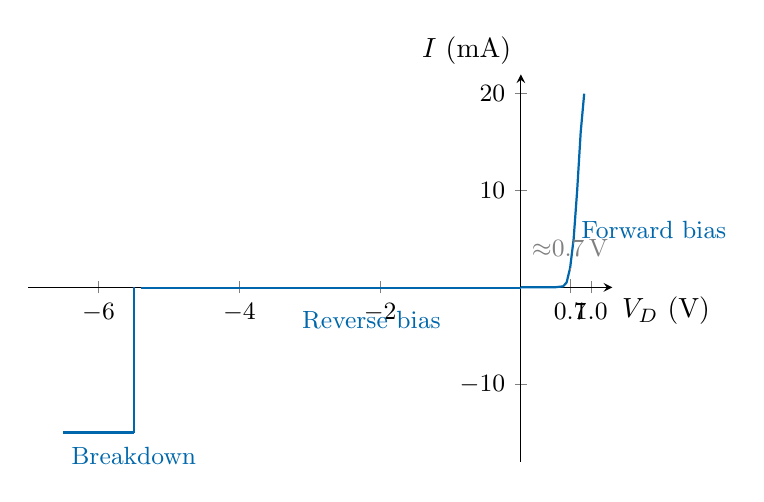
\begin{tikzpicture}
  			\begin{axis}[
  				width=9cm, height=6.5cm,
  				axis lines=center,
  				xlabel={$V_D$ (V)},
  				ylabel={$I$ (mA)},
  				xlabel style={anchor=north west},
  				ylabel style={anchor=south east},
  				xmin=-7, xmax=1.3,
  				ymin=-18, ymax=22,
  				xtick={-6,-4,-2,0,0.7,1.0},
  				xticklabels={$-6$,$-4$,$-2$,$0$,$0.7$,$1.0$},
  				ytick={-10,0,10,20},
  				tick label style={font=\small},
  				clip=false,
  				]
  				\addplot[thick, myblue]
  				coordinates {(-5.4,-0.05)(0,-0.05)};
  				\addplot[thick, myblue]
  				coordinates {
  					(0,0)(0.5,0.02)(0.6,0.1)(0.65,0.5)(0.70,2.0)
  					(0.75,5.0)(0.80,10.0)(0.85,16.0)(0.90,20.0)
  				};
  				\addplot[thick, myblue]
  				coordinates {(-5.5,0)(-5.5,-15)};
  				\addplot[thick, myblue]
  				coordinates {(-5.5,-15)(-6.5,-15)};
  				\addplot[dashed, gray, thin] coordinates {(0.7,0)(0.7,2.0)};
  				\node[font=\small, myblue, anchor=south west] at (axis cs:0.72,4)
  				{Forward bias};
  				\node[font=\small, myblue, anchor=north east] at (axis cs:-1.0,-1.5)
  				{Reverse bias};
  				\node[font=\small, myblue, anchor=north] at (axis cs:-5.5,-15.5)
  				{Breakdown};
  				\node[font=\small, gray, anchor=south] at (axis cs:0.7,2.2)
  				{${\approx}0.7\,\mathrm{V}$};
  			\end{axis}
  		\end{tikzpicture}
  \caption{Typical IV characteristic of a silicon diode. Current is negligible until the forward voltage reaches approximately 0.7~V, then rises steeply. In reverse bias, current is near zero until breakdown.}
\end{figure}

\clearpage

\noindent\textbf{Label:} \texttt{fig:zener-iv-lab}\\[0.5em]
\begin{figure}[H]
  \centering
  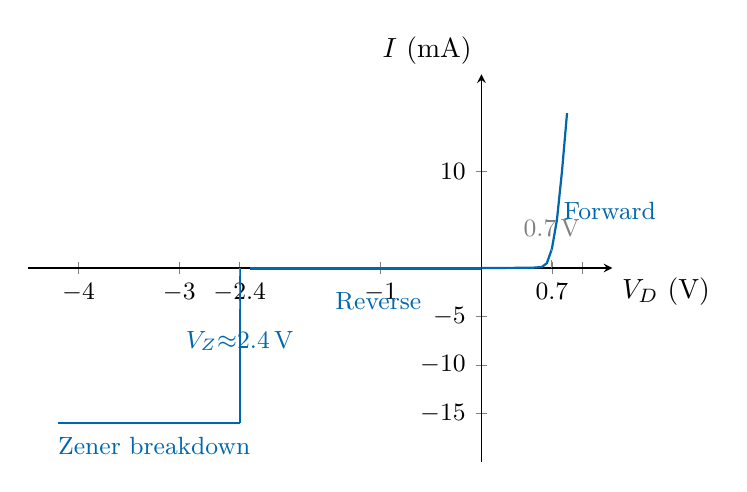
\begin{tikzpicture}
  			\begin{axis}[
  				width=9cm, height=6.5cm,
  				axis lines=center,
  				xlabel={$V_D$ (V)},
  				ylabel={$I$ (mA)},
  				xlabel style={anchor=north west},
  				ylabel style={anchor=south east},
  				xmin=-4.5, xmax=1.3,
  				ymin=-20, ymax=20,
  				xtick={-4,-3,-2.4,-1,0,0.7,1.0},
  				xticklabels={$-4$,$-3$,$-2.4$,$-1$,$0$,$0.7$,{}},
  				ytick={-15,-10,-5,0,10},
  				tick label style={font=\small},
  				clip=false,
  				]
  				\addplot[thick, myblue]
  				coordinates {(-2.3,-0.05)(0,-0.05)};
  				\addplot[thick, myblue]
  				coordinates {
  					(0,0)(0.5,0.02)(0.6,0.1)(0.65,0.5)(0.70,2.0)
  					(0.75,5.0)(0.80,10.0)(0.85,16.0)
  				};
  				\addplot[thick, myblue]
  				coordinates {(-2.4,0)(-2.4,-16)};
  				\addplot[thick, myblue]
  				coordinates {(-2.4,-16)(-4.2,-16)};
  				\addplot[dashed, gray, thin] coordinates {(0.7,0)(0.7,2.0)};
  				\addplot[dashed, gray, thin] coordinates {(-2.4,0)(-2.4,-5)};
  				\node[font=\small, myblue, anchor=south west] at (axis cs:0.72,4)
  				{Forward};
  				\node[font=\small, myblue, anchor=north east] at (axis cs:-0.5,-1.5)
  				{Reverse};
  				\node[font=\small, myblue, anchor=north west] at (axis cs:-4.3,-16.5)
  				{Zener breakdown};
  				\node[font=\small, gray, anchor=south] at (axis cs:0.7,2.2)
  				{$0.7\,\mathrm{V}$};
  				\node[font=\small, myblue, anchor=north] at (axis cs:-2.4,-5.5)
  				{$V_Z{\approx}2.4\,\mathrm{V}$};
  			\end{axis}
  		\end{tikzpicture}
  \caption{IV characteristic of a Zener diode. The forward region is the same as a standard diode. In reverse bias, current is negligible until the Zener voltage $V_Z$ is reached, at which point the device clamps the voltage.}
\end{figure}

\clearpage

\noindent\textbf{Label:} \texttt{fig:iv-circuit-planning}\\[0.5em]
\begin{figure}[H]
  \centering
  \begin{circuitikz}[american]
  			\ctikzset{bipoles/oscope/waveform=none}
  			\draw (0,0) node[ground]{} to[vsourcetri] ++(0,3)
  			to[empty diode] ++ (4,0) to[R=$1 k\Omega$] ++ (0,-3)
  			node[ground]{};
  			\draw (1,3) to[short, *-] ++ (0,2)
  			to[oscope] ++(2,0)
  			to[short, -*] ++ (0,-2);
  			\draw (4,0.5) to[short, *-] ++(2,0) to[oscope] ++(0,2) to[short, -*] ++(-2,0);
  			\node[anchor=south] at (0.5,4) {\textrm{Ch1+}};
  			\node[anchor=south] at (3.5,4) {\textrm{Ch1-}};
  			\node[anchor=south] at (5,2.5) {\textrm{Ch2+}};
  			\node[anchor=south] at (5,2.5-2) {\textrm{Ch2-}};
  		\end{circuitikz}
  \caption{Connection diagram for IV characteristics measurement. CH1 and CH2 are used in XY mode (review the XY mode introduced in Lab~\#2).}
\end{figure}

\clearpage

\noindent\textbf{Label:} \texttt{fig:connection}\\[0.5em]
\begin{figure}[H]
  \centering
  \begin{circuitikz}[american]
  			\ctikzset{bipoles/oscope/waveform=none}
  			\draw (0,0) to[short, -o] ++(1,0)
  			to[short] ++ (1,0)
  			to[vsourcesin] ++(-0,-2)
  			node[ground]{};
  			\draw (0,0) to[oscope] ++(0,-2)
  			node[ground]{};
  			\node[anchor=south] at (-0.6,-0.5) {\textrm{Ch1+}};
  			\node[anchor=south] at (-0.6,-0.3-1.6) {\textrm{Ch1-}};
  			\node[anchor=south] at (2.5,-0.5) {\textrm{W1}};
  			\node[anchor=south] at (2.6,-2.4) {\textrm{\tiny{internal}}};
  		\end{circuitikz}
  \caption{Connection diagram for signal measurement.}
\end{figure}

\clearpage

\noindent\textbf{Label:} \texttt{fig:square\_wave\_spectrum}\\[0.5em]
\begin{figure}[H]
  \centering
  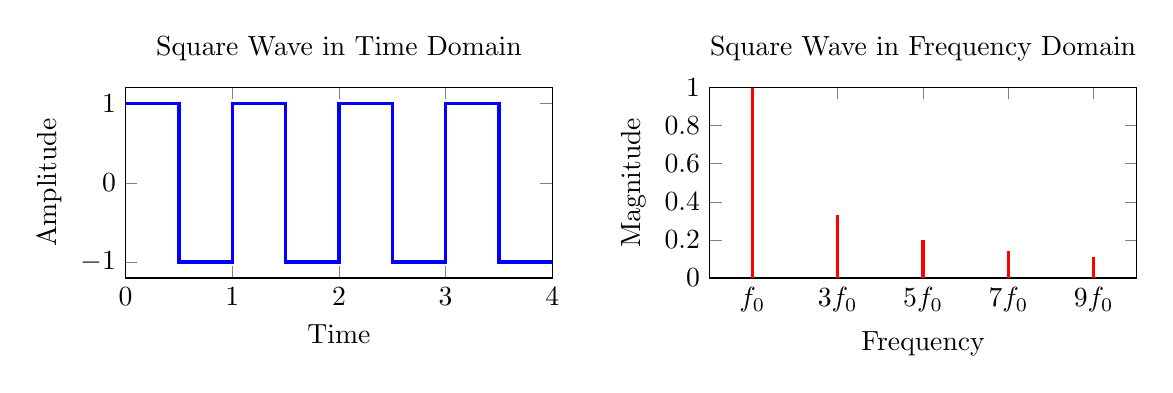
\begin{tikzpicture}
  			\begin{axis}[
  				name=time,
  				title={Square Wave in Time Domain},
  				xlabel={Time},
  				ylabel={Amplitude},
  				xtick={0,1,2,3,4},
  				ytick={-1,0,1},
  				xmin=0, xmax=4,
  				ymin=-1.2, ymax=1.2,
  				width=7cm,
  				height=4cm,
  				]
  				\addplot[very thick, blue, const plot] coordinates {
  					(0, 1) (0.5, 1) (0.5, -1) (1, -1) (1, 1) (1.5, 1) (1.5, -1)
  					(2, -1) (2, 1) (2.5, 1) (2.5, -1) (3, -1) (3, 1) (3.5, 1)
  					(3.5, -1) (4, -1)
  				};
  			\end{axis}
  			\begin{axis}[
  				name=freq,
  				at={($(time.east)+(2cm,0)$)},
  				anchor=west,
  				title={Square Wave in Frequency Domain},
  				xlabel={Frequency},
  				ylabel={Magnitude},
  				xtick={1,3,5,7,9},
  				xticklabels={$f_0$,$3f_0$,$5f_0$,$7f_0$,$9f_0$},
  				ytick={0,0.2,0.4,0.6,0.8,1},
  				xmin=0, xmax=10,
  				ymin=0, ymax=1,
  				width=7cm,
  				height=4cm,
  				]
  				\addplot[very thick, ycomb, red] coordinates {
  					(1, 1) (3, 0.33) (5, 0.2) (7, 0.14) (9, 0.11)
  				};
  			\end{axis}
  		\end{tikzpicture}
  \caption{A square wave in the time domain (left) and frequency domain (right). The spectrum shows the fundamental frequency $f_0$ and odd harmonics ($3f_0$, $5f_0$, etc.) with decreasing amplitudes, illustrating the discrete frequency content of periodic signals.}
\end{figure}

\clearpage

\noindent\textbf{Label:} \texttt{fig:iv-circuit}\\[0.5em]
\begin{figure}[H]
  \centering
  \begin{circuitikz}[american]
  			\ctikzset{bipoles/oscope/waveform=none}
  			\draw (0,0) node[ground]{} to[vsourcetri] ++(0,3)
  			to[european resistor, l_=$DUT$] ++ (4,0) to[R=$1 k\Omega$] ++ (0,-3)
  			node[ground]{};
  			\draw (1,3) to[short, *-] ++ (0,2)
  			to[oscope] ++(2,0)
  			to[short, -*] ++ (0,-2);
  			\draw (4,0.5) to[short, *-] ++(2,0) to[oscope] ++(0,2) to[short, -*] ++(-2,0);
  			\node[anchor=south] at (0.5,4) {\textrm{Ch1+}};
  			\node[anchor=south] at (3.5,4) {\textrm{Ch1-}};
  			\node[anchor=south] at (5,2.5) {\textrm{Ch2+}};
  			\node[anchor=south] at (5,2.5-2) {\textrm{Ch2-}};
  		\end{circuitikz}
  \caption{Circuit connection for IV curve measurement for a Device Under Test (DUT).}
\end{figure}

\end{document}
